\chapter{Разрабатываемый ускоритель}

Ускоритель вычислений - специальное аппаратное устройство, способное выполнять ограниченный ряд задач с большей параллельностью и за меньшее время в сравнении с универсальными микропроцессорными ЭВМ. Топология связей и набор команд примитивных процессорных устройств определяется назначением ускорителя и позволяет высвободить место на кристалле для увеличения их количества. Таким образом достигается большая параллельность работы.

\section{Технология создания ускорителей вычислений}

В данной лабораторной работе изучается технология создания ускорителей вычислений на основе ПЛИС. Основной плат ускорителя Xilinx Alveo U200 является ПЛИС xcu200-fsgd2104-2-e архитектуры Xilinx UltraScale, выполненная по 16-нанометровой технологии. Плата обеспечивает взаимодействие с хост-системой через интерфейс PCIe gen3 x16, и помимо ПЛИС содержит 4 планки памяти DIMM DDR4 по 16 ГБ, и два QSFP разъема для подключения 100ГБ Ethernet сети.

Для работы с ускорительной платой разработано специальное окружение XRT (Xilinx Runtime), включающее компоненты пользовательского пространства и драйвера ядра. XRT поддерживает как карты ускорителей на основе PCIe, так и встроенную архитектуру на основе MPSoC (для встраиваемых плат с ПЛИС Xilinx), обеспечивающую стандартизованный программный интерфейс для Xilinx FPGA.

\section{Архитектура разрабатываемого ускорителя}

В ходе лабораторной работы будет использован базовый шаблон так называемого RTL проекта VINC, который может быть создан в IDE Xilinx Vitis и САПР Xilinx Vivado. Шаблон VINC выполняет попарное сложение чисел исходного массива и сохраняет результаты во втором массиве. Проект VINC включает:

\begin{itemize}
	\item проект ПО хоста, выполняющий инициализацию аппаратного ядра и его тестирование через OpenCL вызовы;
	\item синтезируемый RTL проект ядра ускорителя на языках Verilog и SystemVerilog;
	\item функциональный тест ускорителя VINC на языке SystemVerilog.
\end{itemize}

Функциональная схема разрабатываемой аппаратной системы показана на рисунке \ref{img:scheme}. Проект VINC представляет собой аппаратное устройство, связанное шиной AXI4 MM (Memory mapped) с DDR[i] памятью, и получающее настроечные параметры по интерфейсу AXI4 Lite от программного обеспечения хоста. В рамках всей системы используется единое 64-х разрядное адресное пространство, в котором формируются адреса на всех AXI4 шинах.

В каждой карте U200 имеется возможность подключить ускоритель к любому DDR[i] контроллеру в том регионе, где будет размещен проект. Всего для пользователя доступны 3 динамических региона: SLR0,1,2, для которых выделены каналы локальной памяти DDR[0], DDR[2], DDR[3] соответственно. Вся подключенная память DDR[0..3] доступна со стороны статического региона, в котором размещена аппаратная часть XRT.

Память DDR[1] доступна для использования как в статическом регионе, так и в динамическом регионе SLR1.

Для организации прямого доступа к памяти DDR со стороны хоста также используется AXI4MM шина, соединяющая XDMA PCIe контроллер с контроллером памяти.

Выбор одного из регионов для размещения проектов осуществляется на этапе так называемой линковки конфигурационного файла при помощи компилятора v++(фактически: компоновки, размещение и трассировки нескольких проектов в единый конфигурационный файл).

\begin{figure}[H]
	\begin{center}
		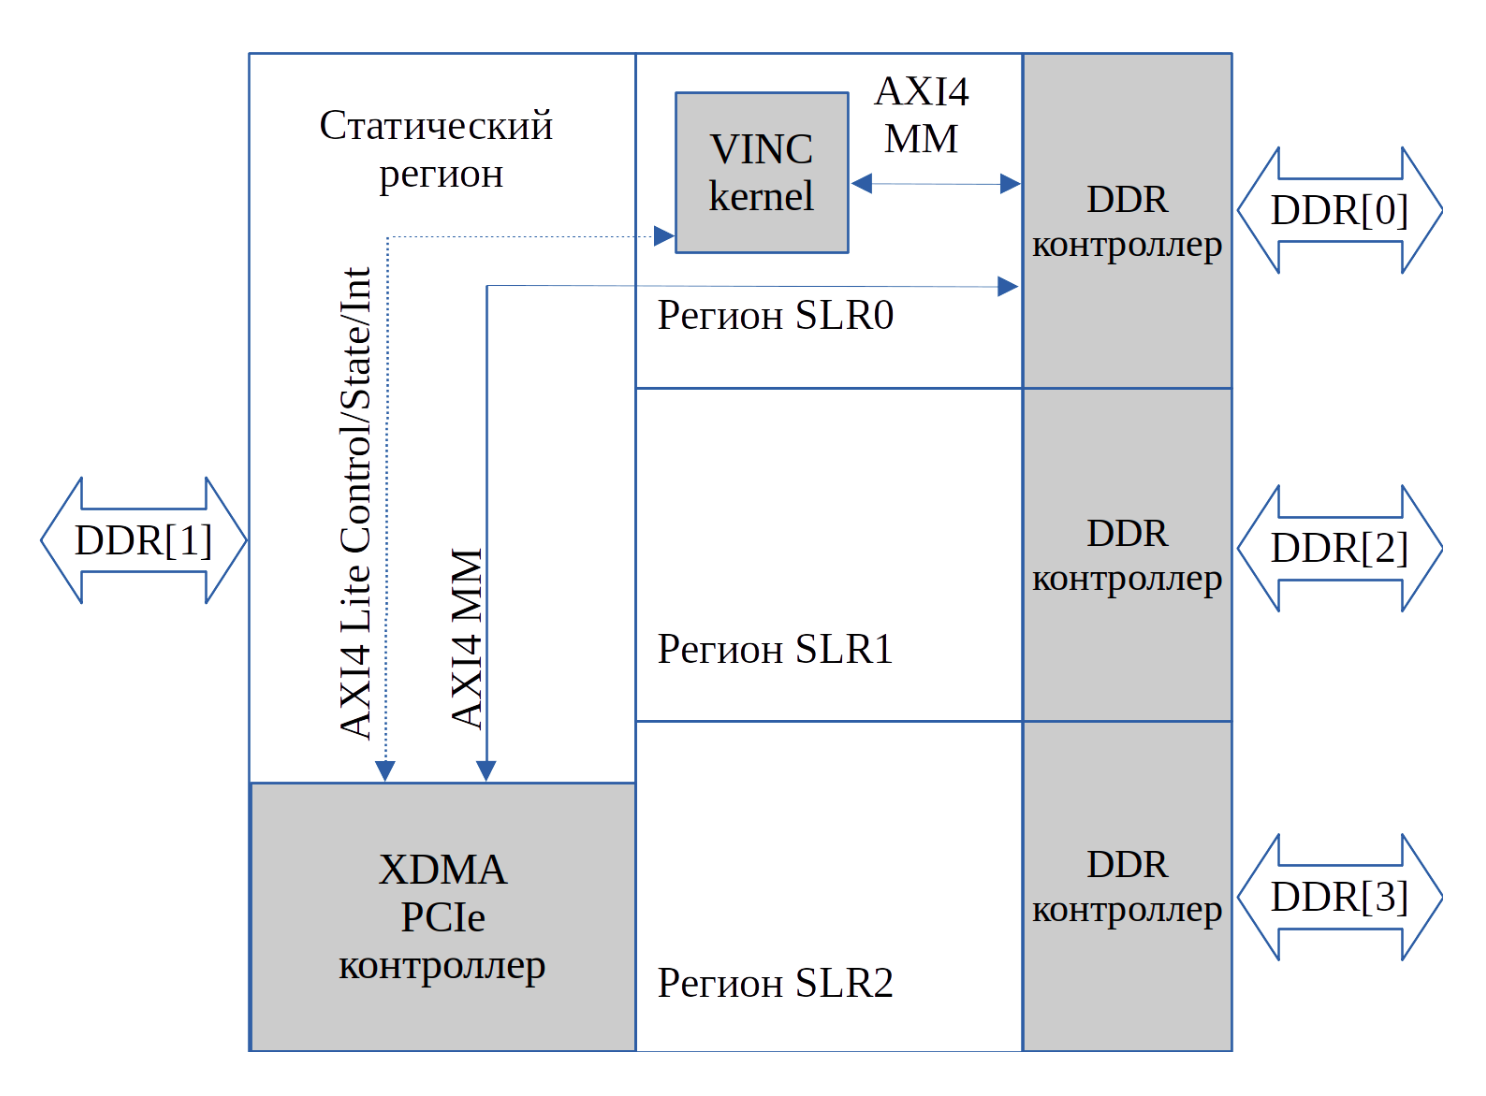
\includegraphics[scale=0.3]{img/scheme.png}
	\end{center}
	\captionsetup{justification=centering}
	\caption{Функциональная схема разрабатываемой аппаратной системы}
	\label{img:scheme}
\end{figure}

\chapter{Моделирование исходного проекта}

На рисунках \ref{img:read}-\ref{img:module_increment} представлены транзакции чтения данных вектора из DDR памяти и записи результата на шине AXI4 MM и инкремент данных в модуле.

\begin{figure}[H]
	\begin{center}
		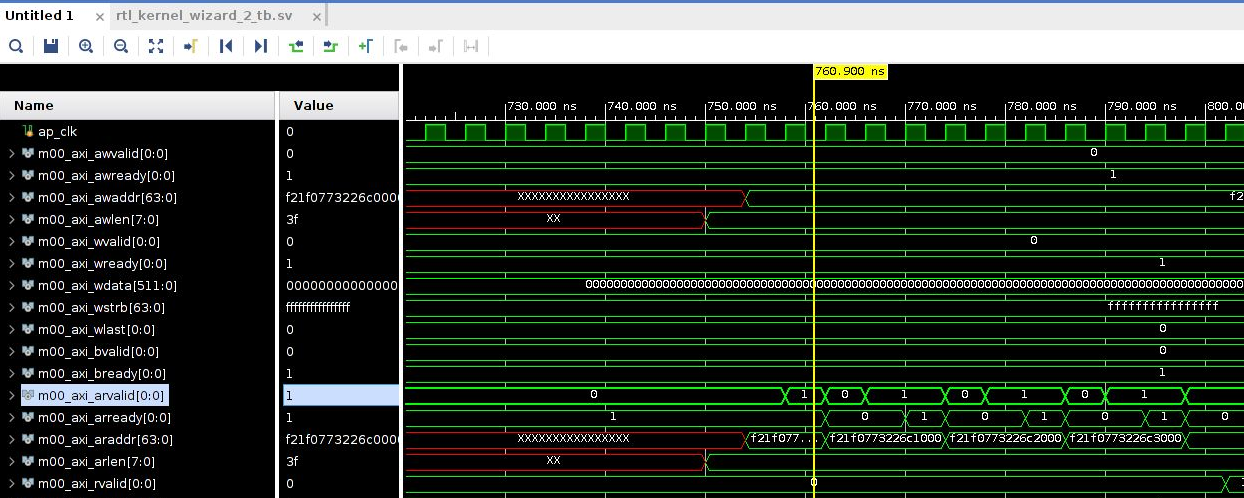
\includegraphics[scale=0.4]{img/read.png}
	\end{center}
	\captionsetup{justification=centering}
	\caption{Транзакция чтения данных вектора на шине AXI4 MM из DDR памяти}
	\label{img:read}
\end{figure}

\begin{figure}[H]
	\begin{center}
		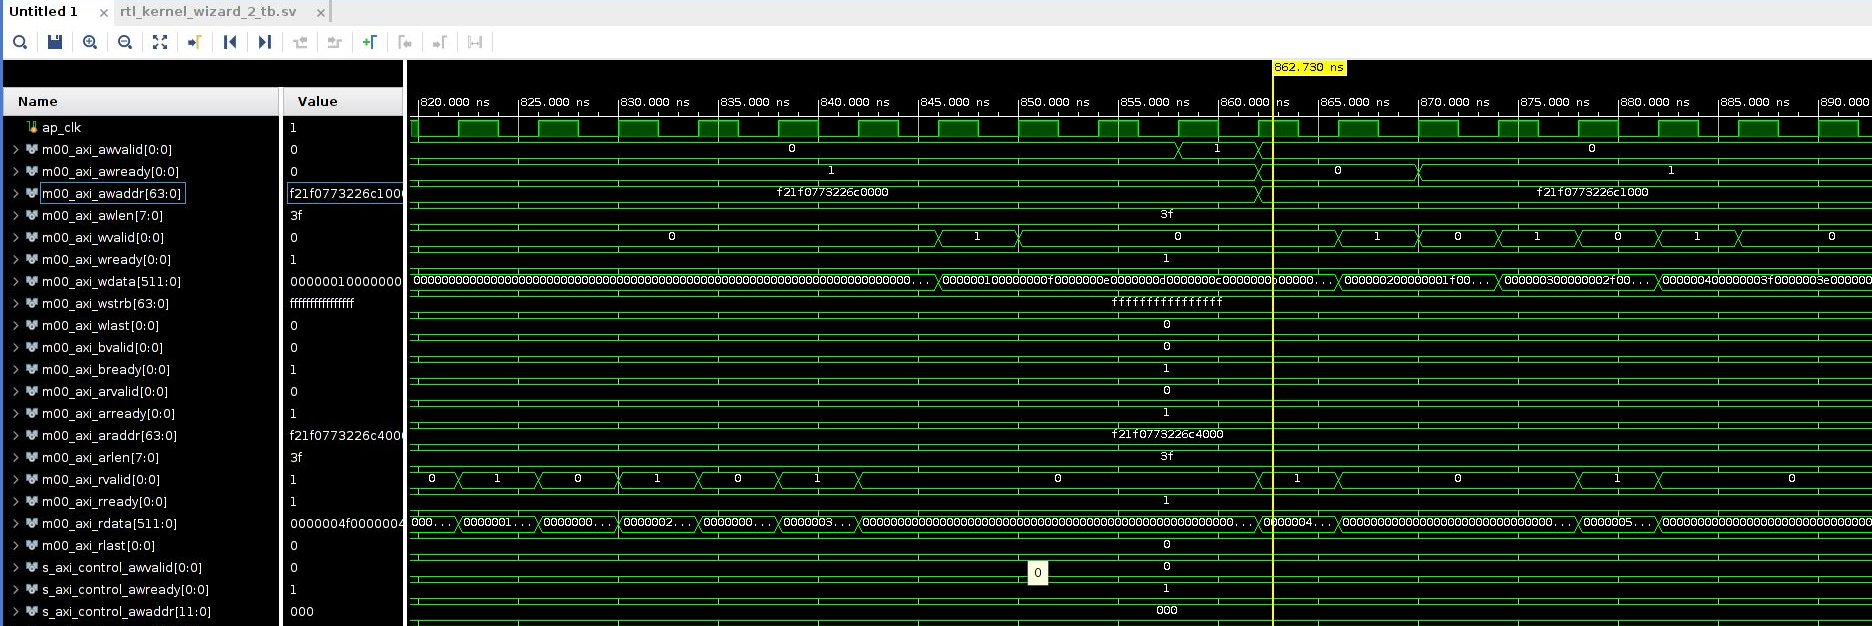
\includegraphics[scale=0.2]{img/increment.png}
	\end{center}
	\captionsetup{justification=centering}
	\caption{Транзакция записи результата инкремента данных на шине AXI4 MM}
	\label{img:increment}
\end{figure}

\begin{figure}[H]
	\begin{center}
		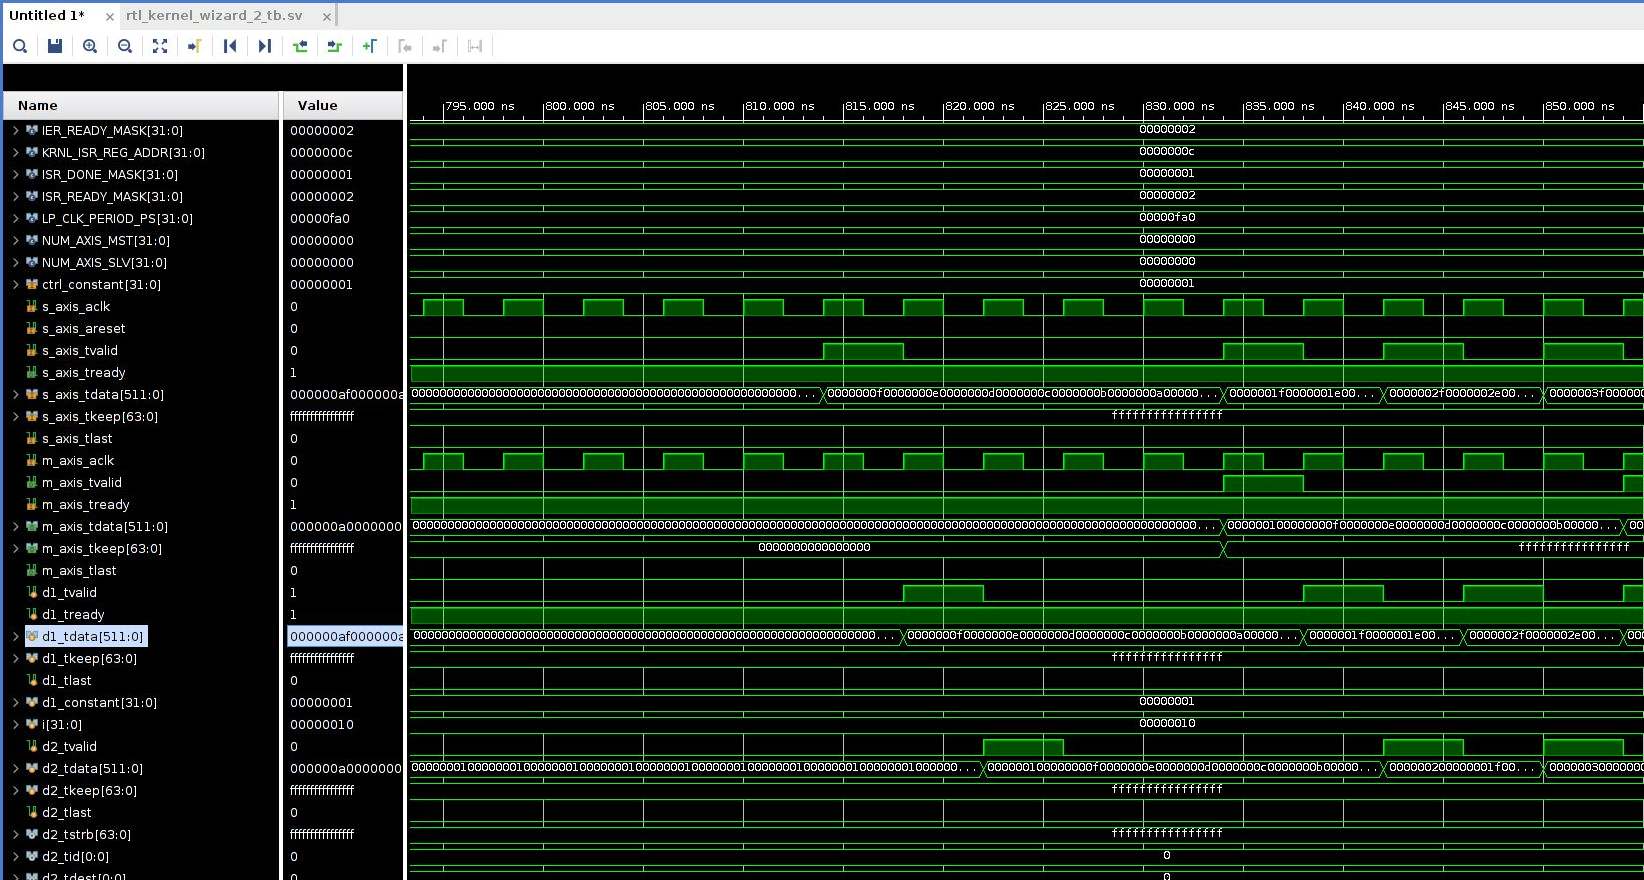
\includegraphics[scale=0.3]{img/module_increment.png}
	\end{center}
	\captionsetup{justification=centering}
	\caption{Инкремент данных в модуле}
	\label{img:module_increment}
\end{figure}

\chapter{Моделирование проекта, измененного по индивидуальному варианту}

В соответствии с вариантом № 18 нужно было реализовать следующую функцию:

\begin{equation}
R[i] = \sim(A[i]+2)
\end{equation}

На рисунке \ref{img:change_func} приведен измененный код, реализующий данную функцию. Для реализации была задана константа $C1 = 2$, которая показана на рисунке \ref{img:const}.

\begin{figure}[H]
	\begin{center}
		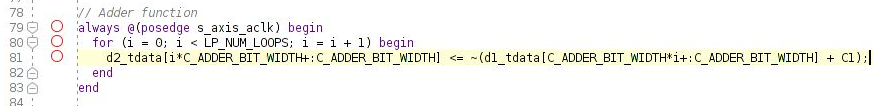
\includegraphics[scale=0.5]{img/change_func.png}
	\end{center}
	\captionsetup{justification=centering}
	\caption{Функция варианта № 18}
	\label{img:change_func}
\end{figure}

\begin{figure}[H]
	\begin{center}
		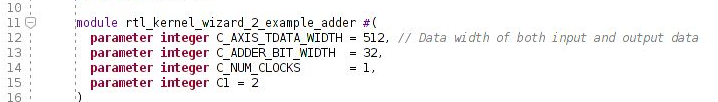
\includegraphics[scale=0.5]{img/const.png}
	\end{center}
	\captionsetup{justification=centering}
	\caption{Константа C1}
	\label{img:const}
\end{figure}

На рисунках \ref{img:new_read}-\ref{img:new_module_increment} представлены транзакции чтения данных вектора из DDR памяти и записи результата на шине AXI4 MM и инкремент данных в модуле.

\begin{figure}[H]
	\begin{center}
		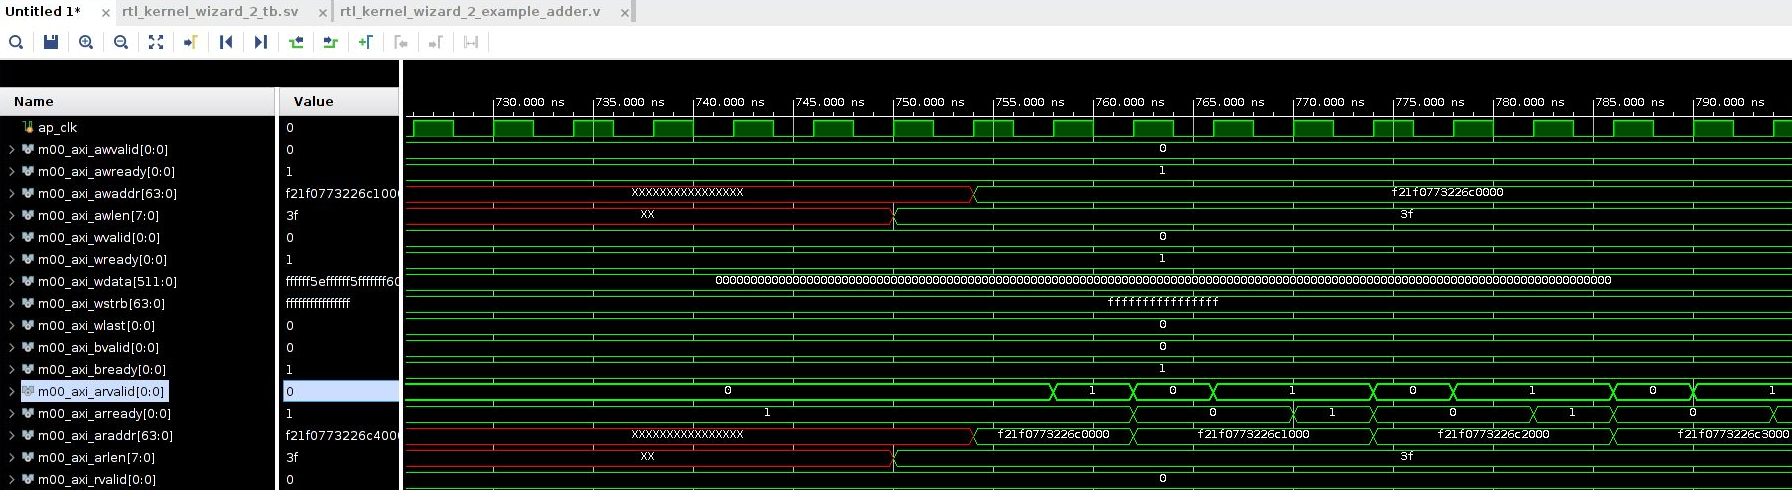
\includegraphics[scale=0.2]{img/new_read.png}
	\end{center}
	\captionsetup{justification=centering}
	\caption{Транзакция чтения данных вектора на шине AXI4 MM из DDR памяти}
	\label{img:new_read}
\end{figure}

\begin{figure}[H]
	\begin{center}
		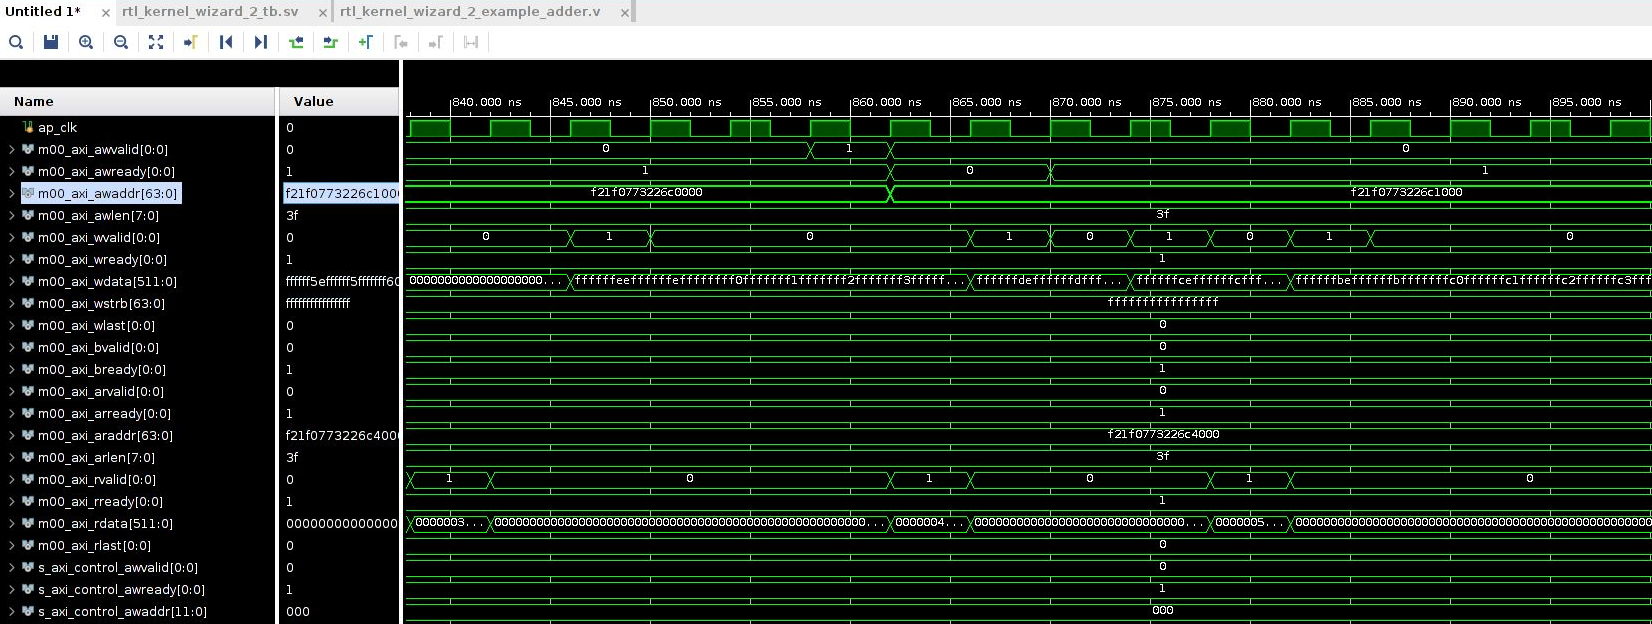
\includegraphics[scale=0.3]{img/new_increment.png}
	\end{center}
	\captionsetup{justification=centering}
	\caption{Транзакция записи результата инкремента данных на шине AXI4 MM}
	\label{img:new_increment}
\end{figure}

\begin{figure}[H]
	\begin{center}
		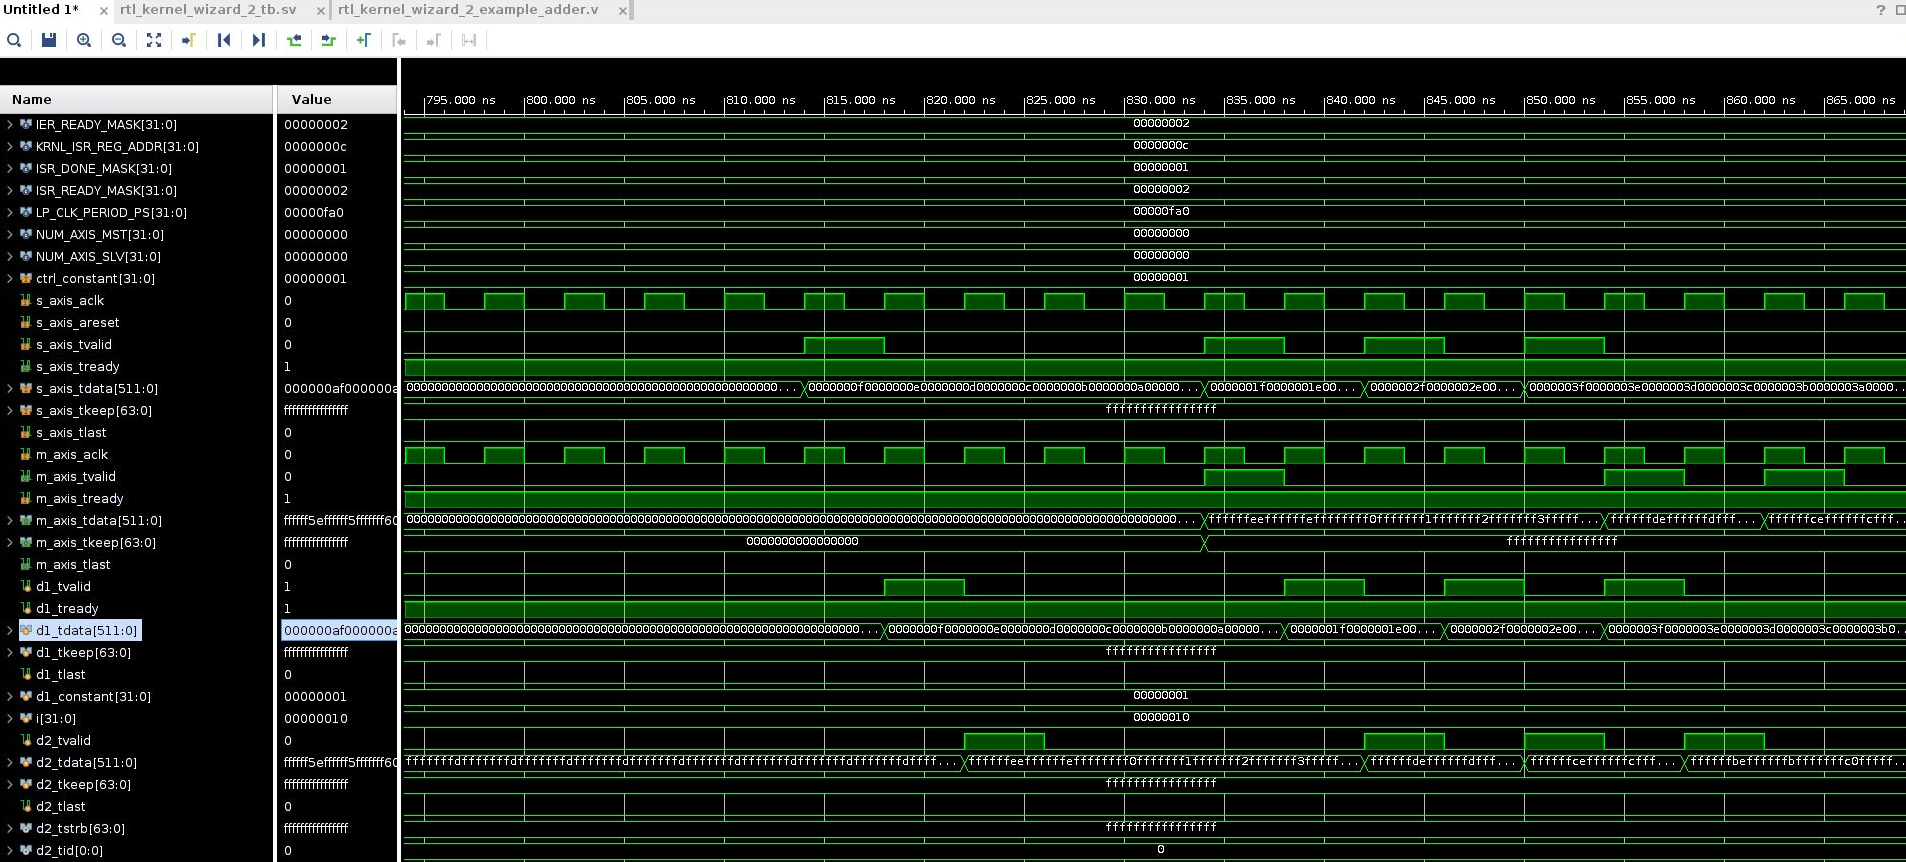
\includegraphics[scale=0.2]{img/new_module_increment.png}
	\end{center}
	\captionsetup{justification=centering}
	\caption{Инкремент данных в модуле}
	\label{img:new_module_increment}
\end{figure}

\chapter{Синтез проекта}

Для синтеза проекта компилятором v++ используется конфигурационный файл $config.cfg$, который содержит основную информацию для работы компилятора:
\begin{itemize}
	\item количество и условные имена экземпляров ядер;
	\item тактовая частота работы ядра;
	\item для каждого ядра: выбор области SLR (SLR[0..2]), выбор DDR (DDR[0..3]) памяти, выбор высокопроизводительной памяти PLRAM(PLRAM[0,1,2]).
	\item параметры синтеза и оптимизации проекта.
\end{itemize}

На рисунке \ref{img:config} представлен конфигурационный файл для данного проекта, в котором в соответствии с вариантом № 18 задан динамический регион $SLR1$ и $DDR[1]$ память.

\begin{figure}[H]
	\begin{center}
		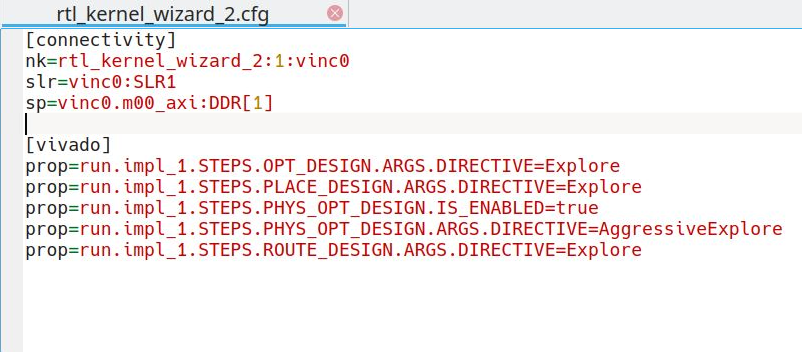
\includegraphics[scale=0.5]{img/config.png}
	\end{center}
	\captionsetup{justification=centering}
	\caption{Конфигурационный файл}
	\label{img:config}
\end{figure}

\textit{Примечание}: листинги файлов $v++*.log$ и $*.xclbin.info$ приведены в приложении.

\chapter{Тестирование}

Для проведения тестирования необходимо изменить файл $host\_example.cpp$ в соответствии с функцией варианта № 18, как показано на рисунке \ref{img:host_example}.

\begin{figure}[H]
	\begin{center}
		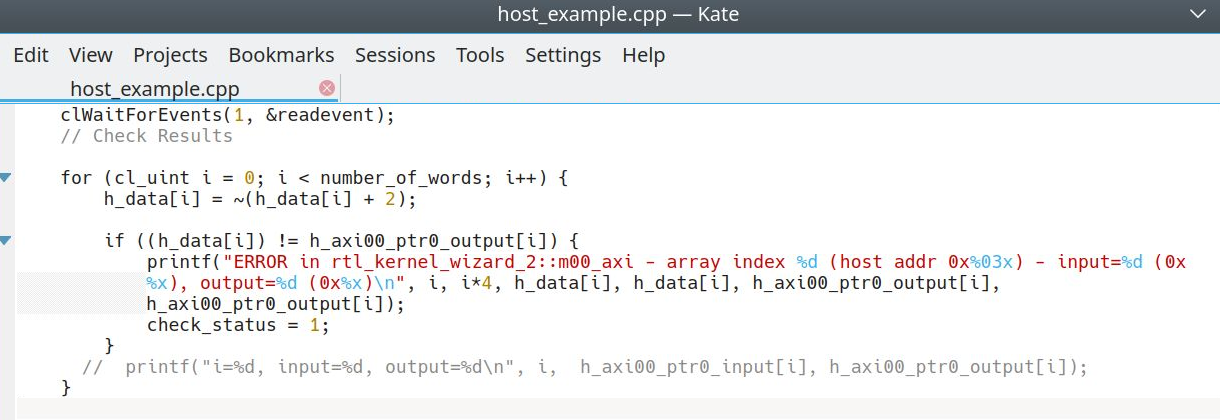
\includegraphics[scale=0.4]{img/host_example.png}
	\end{center}
	\captionsetup{justification=centering}
	\caption{Измененная проверка при тестировании}
	\label{img:host_example}
\end{figure}

Результаты успешного тестирования приведены на рисунке \ref{img:test}.

\begin{figure}[H]
	\begin{center}
		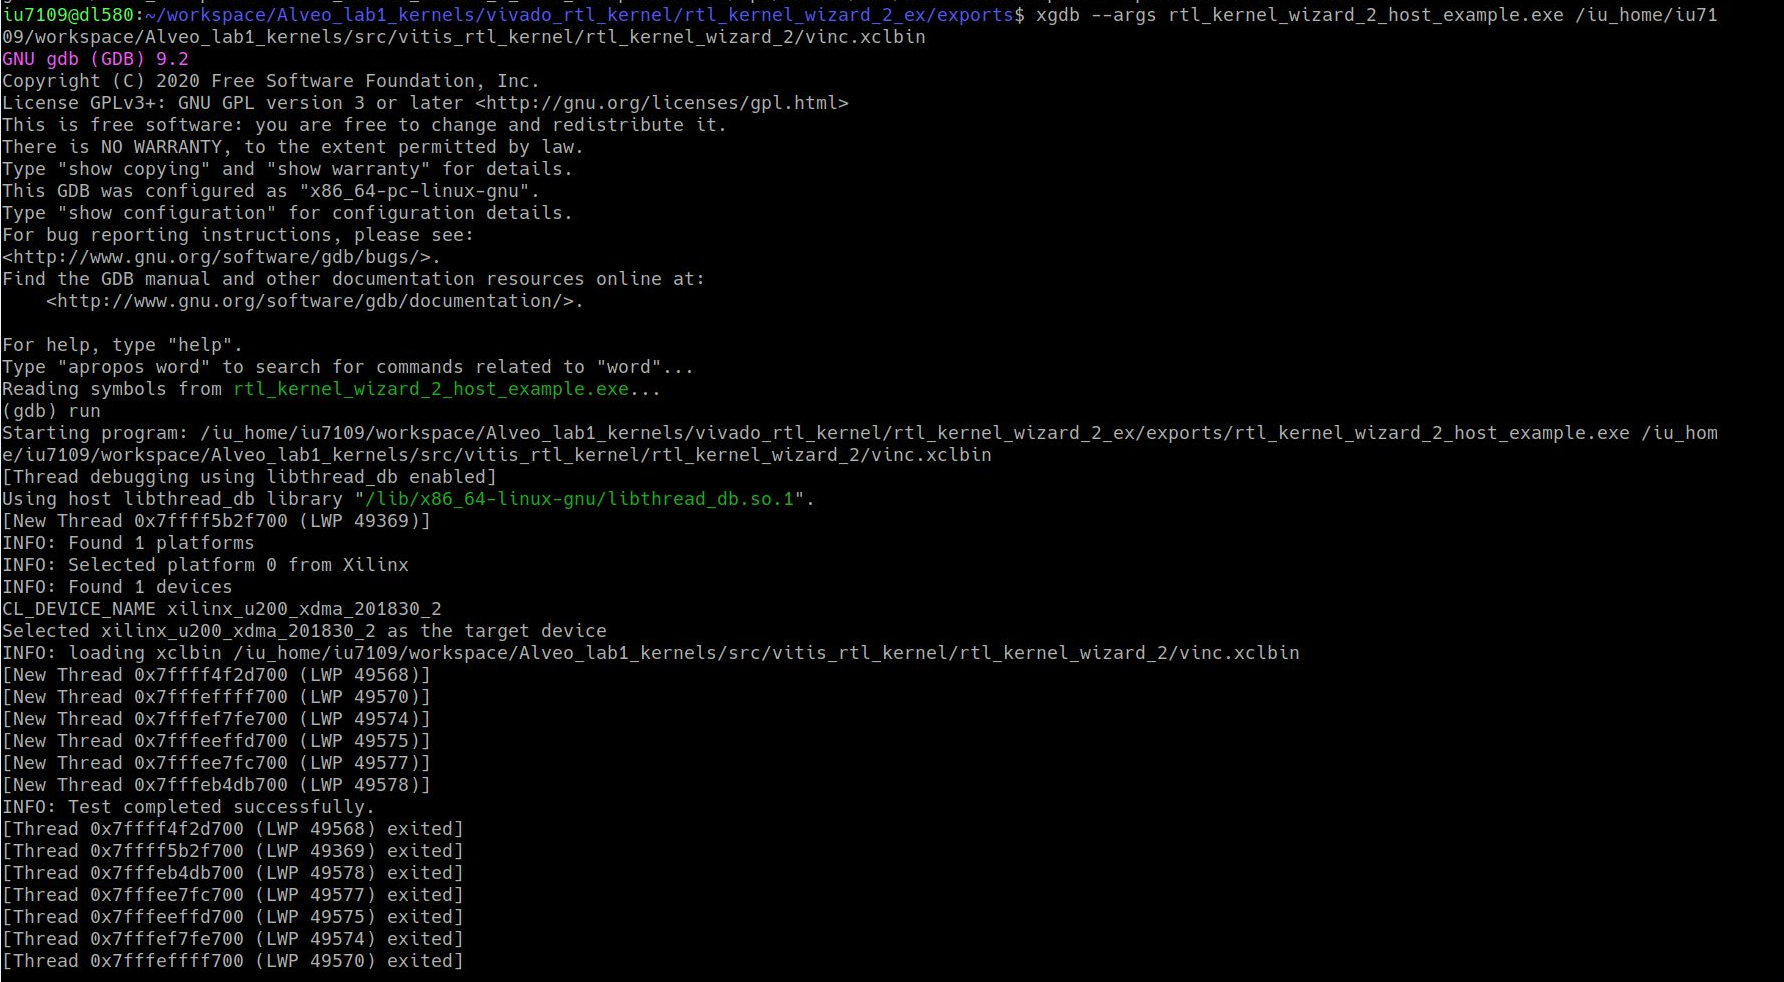
\includegraphics[scale=0.2]{img/test.png}
	\end{center}
	\captionsetup{justification=centering}
	\caption{ Результаты тестирования}
	\label{img:test}
\end{figure}

\chapter{Контрольные вопросы}

\textbf{1. Назовите преимущества и недостатки XDMA и QDMA платформ.}

Преимущества QDMA:
\begin{itemize}
	\item позволяет передавать поток данных непосредственно в логику FPGA параллельно с их обработкой;
	\item высокая производительность;
	\item низкая задержка между хостом и ядрами.
\end{itemize}

Недостатки XDMA:
\begin{itemize}
	\item требует, чтобы данные сначала были полностью перемещены из памяти хоста в память FPGA (DDRx4 DIMM или PLRAM), прежде чем логика FPGA сможет начать обработку данных.
\end{itemize}

\textbf{2. Назовите последовательность действий, необходимых для инициализации ускорителя со стороны хост-системы.}

\begin{itemize}
	\item хост получает все платформы;
 	\item хост выбирает имя платформы Xilinx;
	\item хост получает Id устройства;
	\item хост получает информацию об устройстве;
	\item создается контекст для переменных;
	\item создается команда для ускорителя.
\end{itemize}

\textbf{3. Какова процедура запуска задания на исполнения в ускорительном ядре VINC.}

\begin{itemize}
	\item пользовательское ПО сканирует и инициализирует доступные ускорительные платы, совместимые с XRT, определяет доступные ресурсы, создает программное окружение пользовательского аппаратного ядра ускорителя;
 	\item ресурсы локальной памяти ускорительной платы отображаются в пространство памяти хост системы;
	\item инициализируются каналы DMA для прямого доступа к памяти ускорителя;
	\item данные, подлежащие обработке, копируются из ОЗУ в локальную память ускорителя посредством DMA;
	\item ядру ускорителя посредством записи управляющих
регистров, передаются параметры вычислений;
	\item хост-система выдает сигнал Start ядрам ускорителей, после чего начинается обработка внутри платы Xilinx Alveo.
\end{itemize}

\textbf{4. Опишите процесс линковки на основании содержимого файла v++ *.log.}

\begin{itemize}
	\item анализ профиля устройства. Анализ конфигурационного файла. Поиск необходимых интерфейсов;
	\item FPGA linking synthesized kernels to platform;
	\item оптимизация логики ПЛИС для минимизации задержки;
	\item размещение логики ПЛИС, то есть выбор конкретного места для определенного логического блока;
	\item маршрутизация ПЛИС;
	\item генерация битового потока ПЛИС, то есть
генерация файла [*.xclbin].
\end{itemize}
